\documentclass[12pt]{scrartcl}

\usepackage[utf8]{inputenc}
\usepackage[T1]{fontenc}
\usepackage{lmodern}
\usepackage{graphicx}
\usepackage[pdftex,hyperref,dvipsnames]{xcolor}
\usepackage{listings}
\usepackage[a4paper,lmargin={2cm},rmargin={2cm},tmargin={3.5cm},bmargin = {2.5cm},headheight = {4cm}]{geometry}
\usepackage{amsmath,amssymb,amstext,amsthm}
% \usepackage[lined,algonl,boxed]{algorithm2e} 
\usepackage{algpseudocode}
\usepackage{tikz}
\usepackage{pgfplots}
\usepackage{hyperref}
\usepackage{url}
\usepackage{tcolorbox}
\usepackage[inline]{enumitem}
\usepackage[headsepline]{scrlayer-scrpage} 

\usetikzlibrary{automata,positioning}

\usepgfplotslibrary{external}
%\tikzexternalize
\pgfplotsset{width=10cm,compat=1.9}
\pgfplotsset{every axis/.style={
    axis line style = thick,
    grid = both,
    tick pos = left,
    tick align = outside,
    tick style = {thick,black},
    fill = blue,
	line width = 2pt,
}}

\lstset{
  basicstyle=\ttfamily\small,
  numbers=left,
  numberstyle=\tiny,
  stepnumber=1,
  numbersep=8pt,
  frame=single,
  breaklines=true,
  columns=fullflexible
}

\lstset{
  language=C,
  basicstyle=\ttfamily\small,
  keywordstyle=\color{blue},
  commentstyle=\color{gray},
  stringstyle=\color{green!60!black},
  numbers=left,
  numberstyle=\tiny,
  stepnumber=1,
  numbersep=8pt,
  frame=single,
  breaklines=true,
  columns=fullflexible
}

\renewcommand{\theenumi}{(\alph{enumi})}
\renewcommand{\labelenumi}{\text{\theenumi}}
\renewcommand{\labelenumii}{(\roman{enumii})} 

\ohead{Mubbel\\
       Jan Theil (3794698)}

\ihead{Reinforcement Learning}

\newcounter{exnum}
\newcommand{\exercise}[1]{\section*{Problem \theexnum\stepcounter{exnum}: #1}}

\begin{document}

\setcounter{exnum}{1}

\exercise{Multi-armed Bandits}

\begin{enumerate}
  \item With probability $1 - \epsilon$ we take the greedy action, with probabilty $\epsilon$ we take a random action.
        The overall probabilty to take the greedy action is therefor $(1 - \epsilon) + \dfrac{\epsilon}{k}$. With $k=2, \epsilon = 0.5$ we get: $(1 - 0.5) + \dfrac{0.5}{2} = 0.75$.
  \item \begin{enumerate}
    \item The $\epsilon$ case definitely occured for time steps 2 and 5 (and 1 by design).
    \item It could have possibly occured on time steps 3 and 4. 
  \end{enumerate}
\end{enumerate}

\exercise{Action Selection Strategies}

\begin{enumerate}
  \item Implementation of greedy():
  \begin{center}
    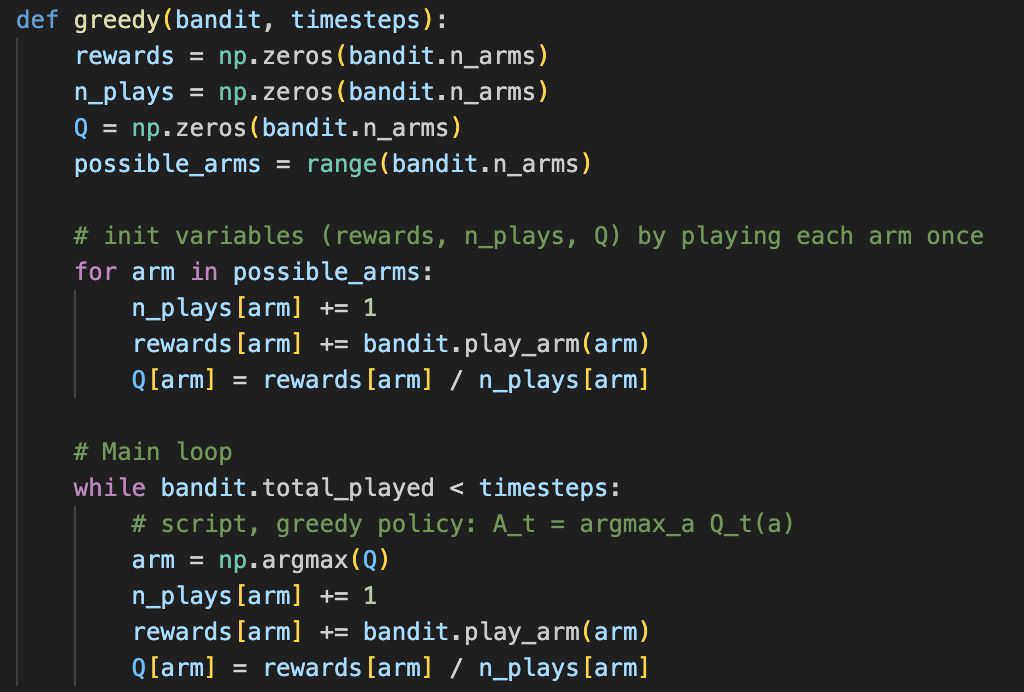
\includegraphics[width=0.5\textwidth]{greedy.png}
  \end{center}

  \item Implementation of epsilon\_greedy():
  \begin{center}
    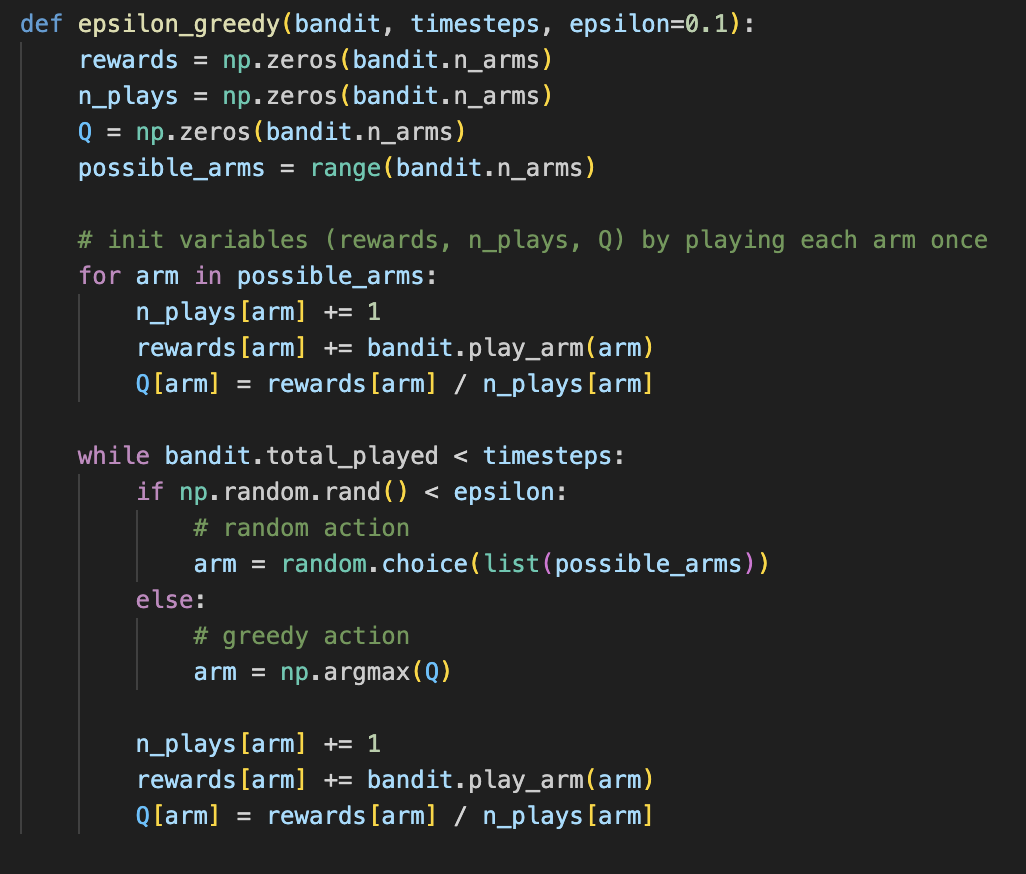
\includegraphics[width=0.5\textwidth]{epsilon_greedy.png}
  \end{center}

  \item greedy() vs epsilon\_greedy():
  \begin{center}
    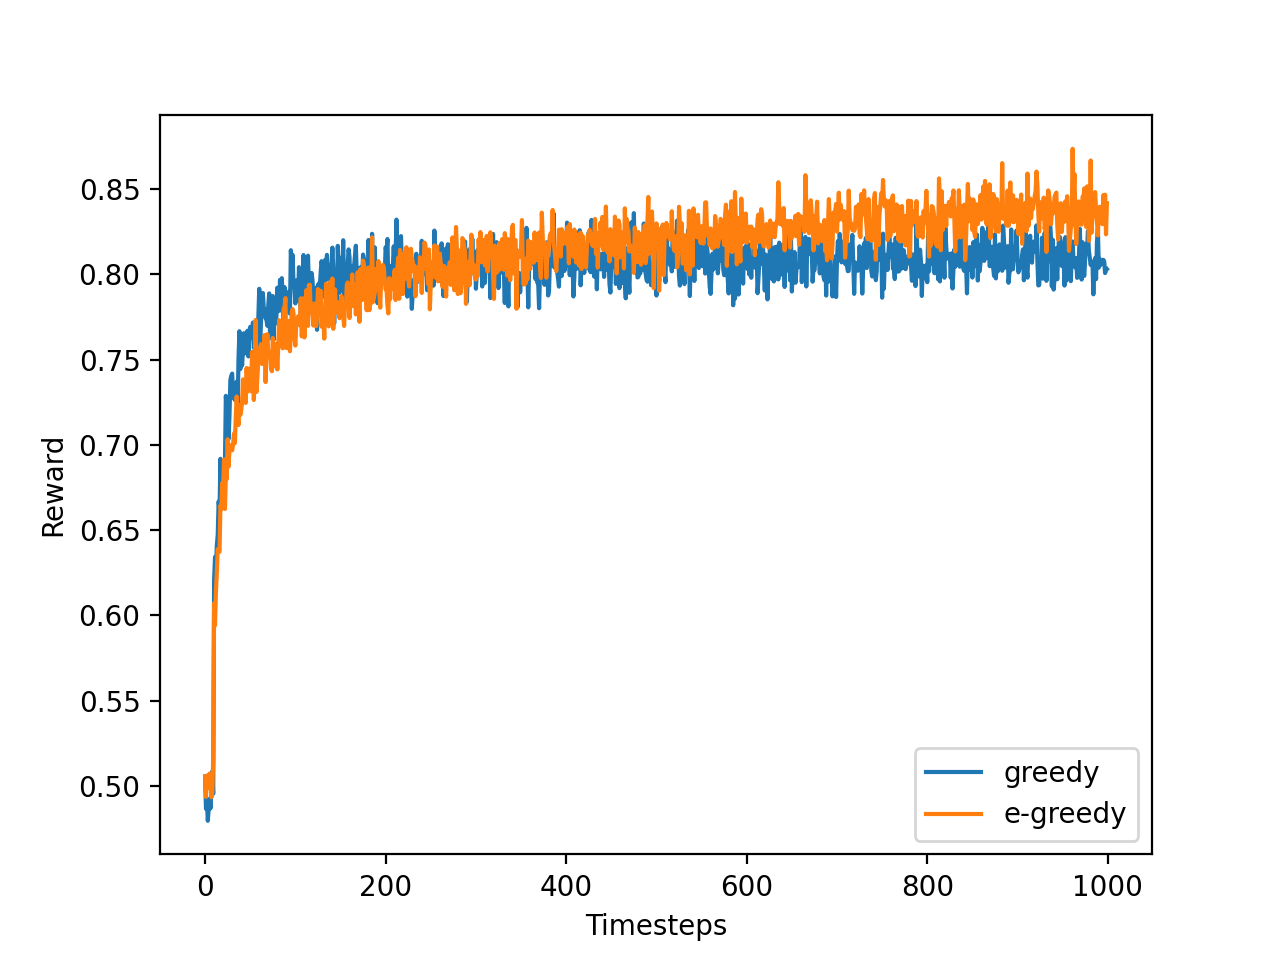
\includegraphics[width=0.5\textwidth]{Figure_1.png}
  \end{center}
        epsilon\_greedy() performs better since the variance of the arm probability distributions is not $0$. Hence not sticking to the first best arm results in a better overall reward.
  \item \begin{enumerate}
    \item One could either manually set another value for $\epsilon$ or let $\epsilon$ change over time.
    \item Initialize $Q$ with non-zero values.
    \item Better exploration by playing 'untouched' arms instead of purely random ones.
  \end{enumerate}
\end{enumerate}

\end{document}